\section{Workflow} \label{subsec:tool_chainv}
Prior to defining how the configuration is specified in \cref{sec:read_input} \nameref{sec:read_input}, we will present the workflow of our solution which provides an overview of how the final system will work.
\Cref{fig:tool1} displays a flowchart representation of the workflow.

\begin{figure}[h]
	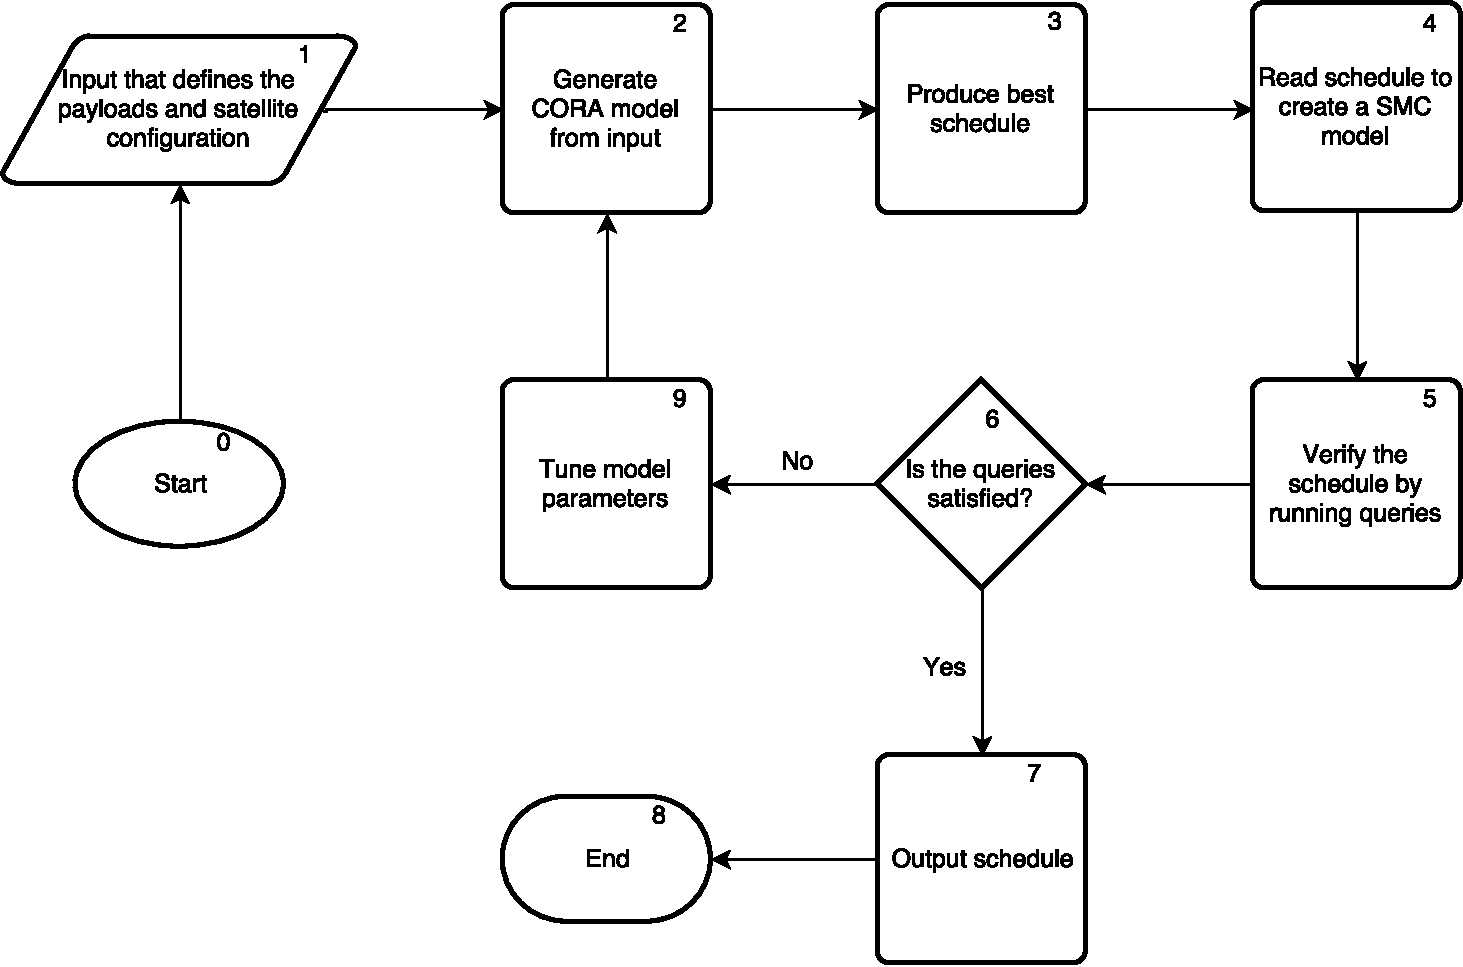
\includegraphics[width=\textwidth]{graphics/flow_final.pdf}
	\caption{Flowchart that displays the workflow}
	\label{fig:tool1}
\end{figure}

\paragraph{Location 1 - Input that defines the payloads and nanosatellite configuration} 
The configuration for the system is read in order to properly model the nanosatellite and its payloads.

\paragraph{Location 2 - Generate \gls{cora} models from input} 
The payloads, windows, and other variables is modelled in the \gls{cora} model, as specified by the input configuration.

\paragraph{Location 3 - Produce best schedule} 
Make \gls{cora}  produce a optimal schedule.

\paragraph{Location 4 - Read schedule to generate a \gls{smc} model}
The model is able to simulate the execution of the schedule and test its robustness.

\paragraph{Location 5 - Verify the schedule by running queries} 
\gls{smc} will run the queries on the model and output the results.
These queries is made to validate and test the robustness of the schedule.

\paragraph{Location 7 - Output schedule} 
The satisfied queries indicate that the schedule is valid, and it will therefore be outputted.

\paragraph{Location 9 - Tune model parameters} 
If the queries were not satisfied, the schedule will be discarded and a new one will be produced.
In order to produce a new schedule, we will provide \gls{cora} with a new configuration.
The configuration will be loyal to the one specified by the user, but certain values will be changed, such as the time to complete a payload, in order to provoke new choices in the scheduler.
